\subsection{Captcha Generator and Preprocessing} \label{section: Captcha_generator}
A key success factor for deep learning system is large amount of data to train.
Intuitively, the simple yet direct approach in data collecting is to mine the captchas from target websites and then paid to mark the labels to them artificially. Obviously, it is a time- or financial-consuming work with a high error rate during manually marking labels.
Further, some websites limit the accessing frequency, making it hard to mine their captchas.
In addition, there is never such a public captcha generator which can produce enough different styles of captchas that match the requirement of the training process.
Thus, the first concern of our work is to develop a flexible, well-calibrated training data generator.

\noindent \textbf{Generative Model:} To generate enough training samples, we design an generation model to imitate captchas production process, and automatically generate different styles of captchas that are similar to those deployed in real-world websites.
Given a unique text-based captcha scheme $x$, we first manually analyze the number of the characters and their corresponding security features, $S_{1:N}$, with $N$ parameters such as font style, size and color, rotating, distortion and waving \emph{et al.} described in Section~\ref{section: sccturity_features}.
Here we ranked the security features from No.1 to 10 shown as Table~\ref{table: feature_number}.
We specifics this analysis results as $\{ M, S_{1:N} \}$, where $M$ and $N$ respectively are the number of characters and its styles.
Then given the content of captcha, our generation model is able to automatically produce captchas image $y$, which accords with its style.
We define our generation model as follows:
\begin{equation}\label{equation: generator_model}
  y \mid x \sim G_s(x),    x = \{M, N, L_{1:M}, S_{1:N} \}
\end{equation}

Where $G_s(x)$ is the generation model parameterized by the unique style $s$, that can generate the target captcha image $y$ based on the target captcha scheme $x$. $M$ is the number of characters of $x$ and $L_{1:M}$ represents the content of the characters. For each character, our generation model individually generates corresponding style defined by $S_{1:N}$, because each character on some captchas may have different style.

\begin{figure}
  \centering
  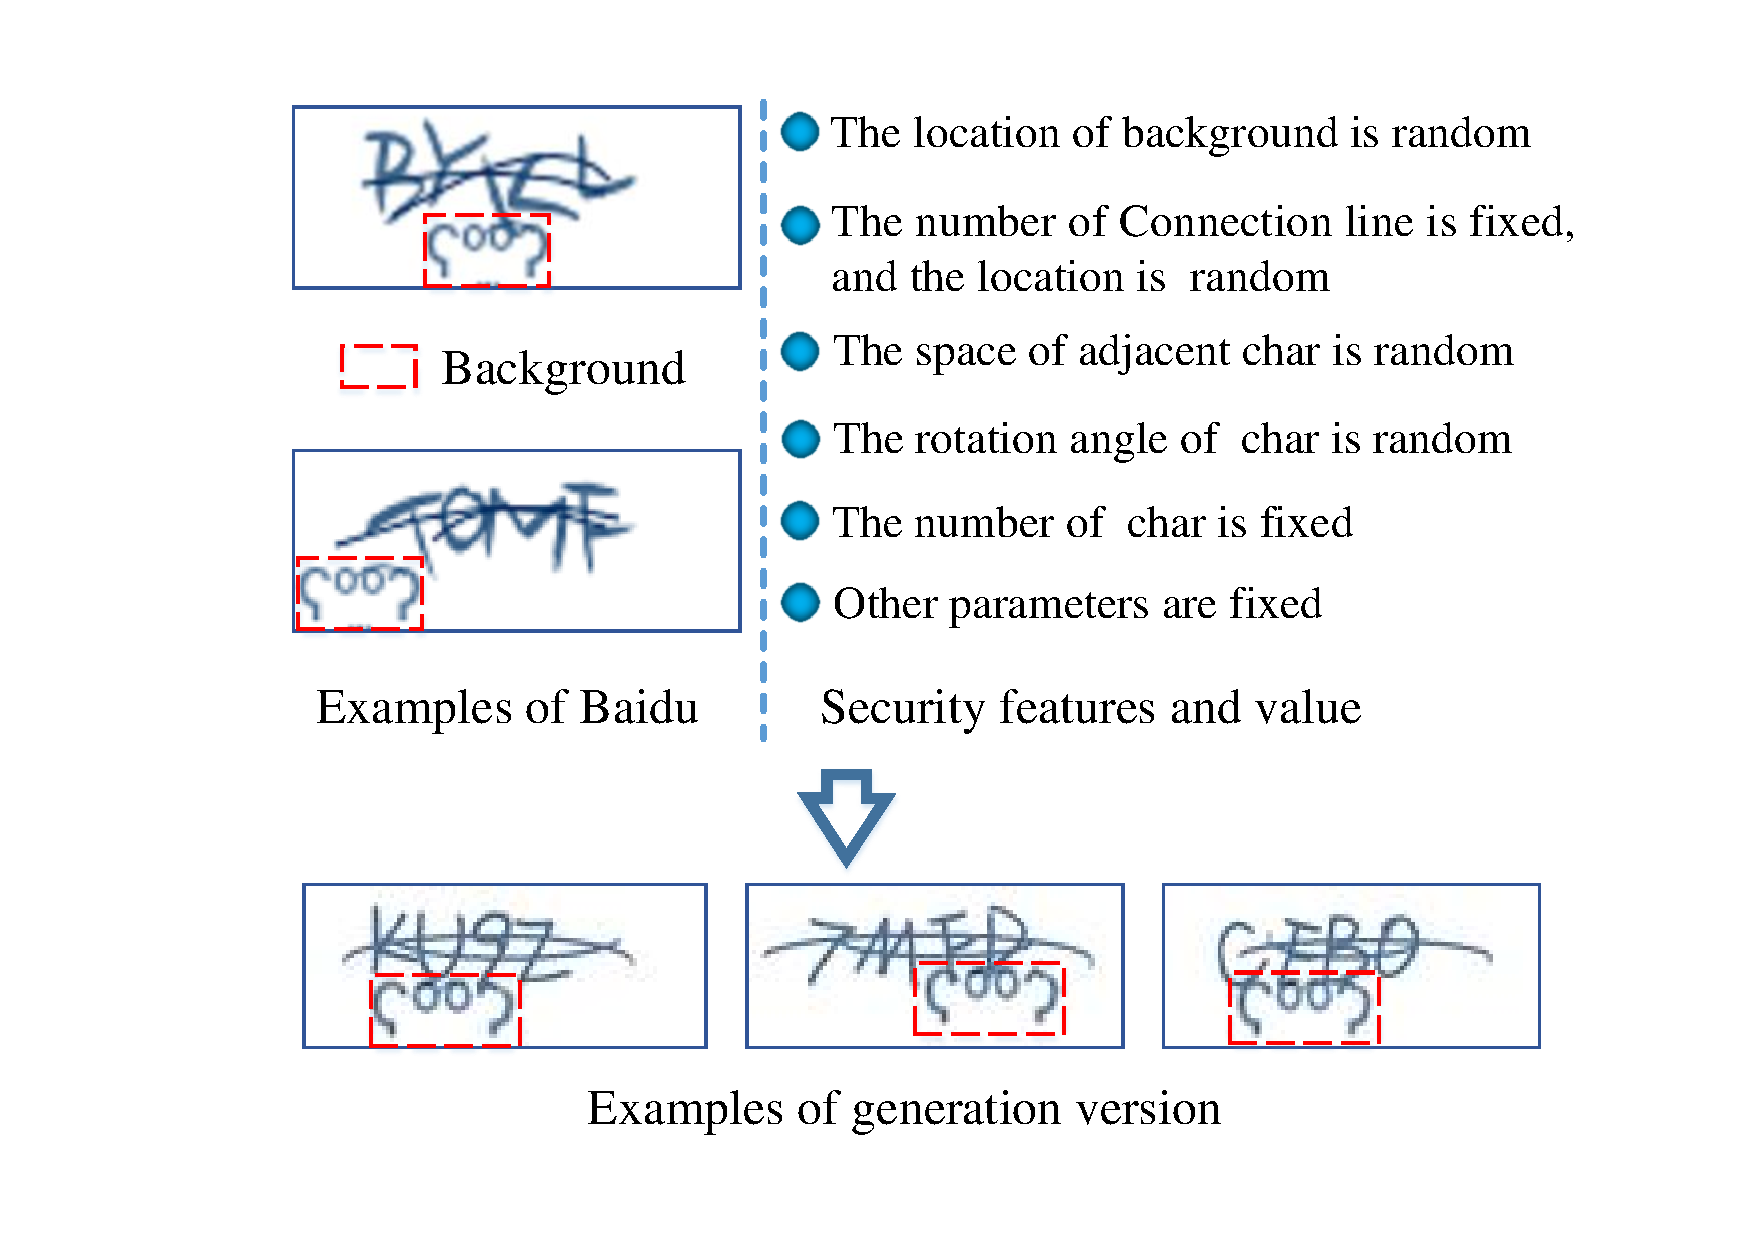
\includegraphics[width=0.47\textwidth]{fig/captcha_analysis/captcha_analysis.pdf}
  \caption{The figure shows the security feature of Baidu Captcha and their parameter value.}
  \label{fig: captcha_analysis}
\end{figure}

\noindent \textbf{Quantify Security Features:} To generate the target captchas as likely as possible, the security features of captcha should be quantified. Given an unique captcha scheme, we first should identify how many security features it used. Then for each used security feature, we need to quantify its parameters value. The last row in Table~\ref{table: feature_number} shows the parameter value for each security feature. For example, if an individual captcha scheme uses rotating and overlapping characters with background, we need to analyze whether the background is fixed or random, the rotating angle and the overlapping distance are fixed or random by observing a number of real captchas. Figure~\ref{fig: captcha_analysis} presents the security features of Baidu captchas and the parameter value of each feature.

\noindent \textbf{Example:} We use the captcha image depicted in Figure~\ref{fig:overview} as an example to describe our captcha generator. This captcha scheme consists of only English letters and Arabic numerals and the number of characters are fixed (4 characters). The content of the captcha is $\{d, 0, a, A\}$.
It uses 3 anti-segmentation features (Complex Background, Connection Lines, overlapping) and 4 anti-recognition features (Character Set, Font size, Rotating and Distortion). So the collection of security features number is \{\circled{\small 0}, \circled{\small 1}, \circled{\small 2}, \circled{\small 3}, \circled{\small 4}, \circled{\small 6}, \circled{\small 7}\}.
Among these security features, we observed that both the location of connection lines and the space of adjacent character are random, and other parameters value of security features are fixed. So the collection of security features can be represented as \emph{SF}: \{\{\circled{\small 0}, f\}, \{\circled{\small 1}, f, r\}, \{\circled{\small 2}, r\}, \{\circled{\small 3}, f\}, \{\circled{\small 4}, f\}, \{\circled{\small 6}, f\}, \{\circled{\small 7}, r\}\}.
Considering these parameters, the variance $x$ is $\{4, 6, \{7, j, R, U\}, \emph{SF}\}$.
For each character in the collection $\{4, 6, \{7, j, R, U\}\}$, our generator product the subgraph correspond to its security features. At last, the generator aggregates the subgraph to produce a captcha image.

